% TO-DO:
% Change subsection titles in the history.tex (You should see a comment about this under the 1st subsection)

\documentclass[10pt,conference]{IEEEtran}
\usepackage{cite}
\usepackage[tight,footnotesize]{subfigure}
% cite.sty was written by Donald Arseneau
% V1.6 and later of IEEEtran pre-defines the format of the cite.sty package
% \cite{} output to follow that of IEEE. Loading the cite package will
% result in citation numbers being automatically sorted and properly
% "compressed/ranged". e.g., [1], [9], [2], [7], [5], [6] without using
% cite.sty will become [1], [2], [5]--[7], [9] using cite.sty. cite.sty's
% \cite will automatically add leading space, if needed. Use cite.sty's
% noadjust option (cite.sty V3.8 and later) if you want to turn this off
% such as if a citation ever needs to be enclosed in parenthesis.
% cite.sty is already installed on most LaTeX systems. Be sure and use
% version 4.0 (2003-05-27) and later if using hyperref.sty. cite.sty does
% not currently provide for hyperlinked citations.
% The latest version can be obtained at:
% http://www.ctan.org/tex-archive/macros/latex/contrib/cite/
% The documentation is contained in the cite.sty file itself.






% *** GRAPHICS RELATED PACKAGES ***
%
\ifCLASSINFOpdf
   \usepackage[pdftex]{graphicx}
  % declare the path(s) where your graphic files are
  % \graphicspath{{../pdf/}{../jpeg/}}
  % and their extensions so you won't have to specify these with
  % every instance of \includegraphics
  % \DeclareGraphicsExtensions{.pdf,.jpeg,.png}
\else
  % or other class option (dvipsone, dvipdf, if not using dvips). graphicx
  % will default to the driver specified in the system graphics.cfg if no
  % driver is specified.
  % \usepackage[dvips]{graphicx}
  % declare the path(s) where your graphic files are
  % \graphicspath{{../eps/}}
  % and their extensions so you won't have to specify these with
  % every instance of \includegraphics
  % \DeclareGraphicsExtensions{.eps}
\fi
% graphicx was written by David Carlisle and Sebastian Rahtz. It is
% required if you want graphics, photos, etc. graphicx.sty is already
% installed on most LaTeX systems. The latest version and documentation
% can be obtained at: 
% http://www.ctan.org/tex-archive/macros/latex/required/graphics/
% Another good source of documentation is "Using Imported Graphics in
% LaTeX2e" by Keith Reckdahl which can be found at:
% http://www.ctan.org/tex-archive/info/epslatex/
%
% latex, and pdflatex in dvi mode, support graphics in encapsulated
% postscript (.eps) format. pdflatex in pdf mode supports graphics
% in .pdf, .jpeg, .png and .mps (metapost) formats. Users should ensure
% that all non-photo figures use a vector format (.eps, .pdf, .mps) and
% not a bitmapped formats (.jpeg, .png). IEEE frowns on bitmapped formats
% which can result in "jaggedy"/blurry rendering of lines and letters as
% well as large increases in file sizes.
%
% You can find documentation about the pdfTeX application at:
% http://www.tug.org/applications/pdftex





% *** MATH PACKAGES ***
%
\usepackage[cmex10]{amsmath}
\usepackage{amssymb}
% A popular package from the American Mathematical Society that provides
% many useful and powerful commands for dealing with mathematics. If using
% it, be sure to load this package with the cmex10 option to ensure that
% only type 1 fonts will utilized at all point sizes. Without this option,
% it is possible that some math symbols, particularly those within
% document that can not be IEEE Xplore compliant!
%
% Also, note that the amsmath package sets \interdisplaylinepenalty to 10000
% thus preventing page breaks from occurring within multiline equations. Use:
%\interdisplaylinepenalty=2500
% after loading amsmath to restore such page breaks as IEEEtran.cls normally
% does. amsmath.sty is already installed on most LaTeX systems. The latest
% version and documentation can be obtained at:
% http://www.ctan.org/tex-archive/macros/latex/required/amslatex/math/





% *** SPECIALIZED LIST PACKAGES ***
%
\usepackage{algorithm}
\usepackage{algorithmic}
% algorithmic.sty was written by Peter Williams and Rogerio Brito.
% This package provides an algorithmic environment fo describing algorithms.
% You can use the algorithmic environment in-text or within a figure
% environment to provide for a floating algorithm. Do NOT use the algorithm
% floating environment provided by algorithm.sty (by the same authors) or
% algorithm2e.sty (by Christophe Fiorio) as IEEE does not use dedicated
% algorithm float types and packages that provide these will not provide
% correct IEEE style captions. The latest version and documentation of
% algorithmic.sty can be obtained at:
% http://www.ctan.org/tex-archive/macros/latex/contrib/algorithms/
% There is also a support site at:
% http://algorithms.berlios.de/index.html
% Also of interest may be the (relatively newer and more customizable)
% algorithmicx.sty package by Szasz Janos:
% http://www.ctan.org/tex-archive/macros/latex/contrib/algorithmicx/




% *** ALIGNMENT PACKAGES ***
%
%\usepackage{array}
% Frank Mittelbach's and David Carlisle's array.sty patches and improves
% the standard LaTeX2e array and tabular environments to provide better
% appearance and additional user controls. As the default LaTeX2e table
% generation code is lacking to the point of almost being broken with
% respect to the quality of the end results, all users are strongly
% advised to use an enhanced (at the very least that provided by array.sty)
% set of table tools. array.sty is already installed on most systems. The
% latest version and documentation can be obtained at:
% http://www.ctan.org/tex-archive/macros/latex/required/tools/


% IEEEtran contains the IEEEeqnarray family of commands that can be used to
% generate multiline equations as well as matrices, tables, etc., of high
% quality.




% *** SUBFIGURE PACKAGES ***
%\ifCLASSOPTIONcompsoc
%  \usepackage[caption=false,font=normalsize,labelfont=sf,textfont=sf]{subfig}
%\else
%  \usepackage[caption=false,font=footnotesize]{subfig}
%\fi
% subfig.sty, written by Steven Douglas Cochran, is the modern replacement
% for subfigure.sty, the latter of which is no longer maintained and is
% incompatible with some LaTeX packages including fixltx2e. However,
% subfig.sty requires and automatically loads Axel Sommerfeldt's caption.sty
% which will override IEEEtran.cls' handling of captions and this will result
% in non-IEEE style figure/table captions. To prevent this problem, be sure
% and invoke subfig.sty's "caption=false" package option (available since
% subfig.sty version 1.3, 2005/06/28) as this is will preserve IEEEtran.cls
% handling of captions.
% Note that the Computer Society format requires a larger sans serif font
% than the serif footnote size font used in traditional IEEE formatting
% and thus the need to invoke different subfig.sty package options depending
% on whether compsoc mode has been enabled.
%
% The latest version and documentation of subfig.sty can be obtained at:
% http://www.ctan.org/tex-archive/macros/latex/contrib/subfig/




% *** FLOAT PACKAGES ***
%
%\usepackage{fixltx2e}
% fixltx2e, the successor to the earlier fix2col.sty, was written by
% Frank Mittelbach and David Carlisle. This package corrects a few problems
% in the LaTeX2e kernel, the most notable of which is that in current
% LaTeX2e releases, the ordering of single and double column floats is not
% guaranteed to be preserved. Thus, an unpatched LaTeX2e can allow a
% single column figure to be placed prior to an earlier double column
% figure. The latest version and documentation can be found at:
% http://www.ctan.org/tex-archive/macros/latex/base/


%\usepackage{stfloats}
% stfloats.sty was written by Sigitas Tolusis. This package gives LaTeX2e
% the ability to do double column floats at the bottom of the page as well
% as the top. (e.g., "\begin{figure*}[!b]" is not normally possible in
% LaTeX2e). It also provides a command:
%\fnbelowfloat
% to enable the placement of footnotes below bottom floats (the standard
% LaTeX2e kernel puts them above bottom floats). This is an invasive package
% which rewrites many portions of the LaTeX2e float routines. It may not work
% with other packages that modify the LaTeX2e float routines. The latest
% version and documentation can be obtained at:
% http://www.ctan.org/tex-archive/macros/latex/contrib/sttools/
% Do not use the stfloats baselinefloat ability as IEEE does not allow
% \baselineskip to stretch. Authors submitting work to the IEEE should note
% that IEEE rarely uses double column equations and that authors should try
% to avoid such use. Do not be tempted to use the cuted.sty or midfloat.sty
% packages (also by Sigitas Tolusis) as IEEE does not format its papers in
% such ways.
% Do not attempt to use stfloats with fixltx2e as they are incompatible.
% Instead, use Morten Hogholm'a dblfloatfix which combines the features
% of both fixltx2e and stfloats:
%
% \usepackage{dblfloatfix}
% The latest version can be found at:
% http://www.ctan.org/tex-archive/macros/latex/contrib/dblfloatfix/




% *** PDF, URL AND HYPERLINK PACKAGES ***
%
\usepackage{url}
% url.sty was written by Donald Arseneau. It provides better support for
% handling and breaking URLs. url.sty is already installed on most LaTeX
% systems. The latest version and documentation can be obtained at:
% http://www.ctan.org/tex-archive/macros/latex/contrib/url/
% Basically, \url{my_url_here}.




% *** Do not adjust lengths that control margins, column widths, etc. ***
% *** Do not use packages that alter fonts (such as pslatex).         ***
% There should be no need to do such things with IEEEtran.cls V1.6 and later.
% (Unless specifically asked to do so by the journal or conference you plan
% to submit to, of course. )

% THIS IS DEFINITELY WORTH NOTING
% correct bad hyphenation here
\hyphenation{op-tical net-works semi-conduc-tor}

\begin{document}
%
% paper title
% can use linebreaks \\ within to get better formatting as desired
%\title{DC-AFCD: a Fair and Low Latency AQM Scheme for Data Center Switches}
\title{Network Security and Preventive Measures in the Age of Big data}
% author names and affiliations
% use a multiple column layout for up to three different
% affiliations
  \author{\IEEEauthorblockN{Forrest Bankston, William Kane, Suman Kumar}
    \IEEEauthorblockA{Department of Computer Science, Troy University, Troy, AL, USA, 36082\\
Email: \{jbankston, wkane, skumar\}@troy.edu
 }} % WK Please put your email in place here and delete this comment in your commit

% make the title area
\maketitle

\begin{abstract}
%This could definitely use some editing + extra information
Over time, Big Data has evolved to become one of the key components for enterprise growth. Big Data structures allow for organizations to process and operate upon massive amounts of data in order to make better business decisions and find hidden patterns within the data. Such data will often be sensitive and require a platform built for efficient and secure delivery. Therefore, network security should always be at the forefront of concerns when dealing when any type of Big Data scheme. Network security in this context faces some unique challenges because of the unique systems and adaptations created to support Big Data. This paper will give an introduction to Big Data systems and the unique kinds of challenges and attacks they face. The paper will then give a survey over the common and standard prevention mechanisms that are employed to protect our sensitive Big Data schemes.
%These inputs contain the text which you will see in the document
%They are found in the subtex directory of the project folder
\end{abstract}
\begin{IEEEkeywords}
Network Security, Big Data, etc., More Keywords Here\end{IEEEkeywords}

% no keywords




% For peer review papers, you can put extra information on the cover
% page as needed:
% \ifCLASSOPTIONpeerreview
% \begin{center} \bfseries EDICS Category: 3-BBND \end{center}
% \fi
%
% For peerreview papers, this IEEEtran command inserts a page break and
% creates the second title. It will be ignored for other modes.
\IEEEpeerreviewmaketitle



\section{Introduction}
\label{intro}
% Many of these labels need to be fixed in the subtex
Cloud computing is the concept of computing remotely through Internet on data centers where thousands of computers/server and other communication devices are installed and running 24/7. Now-a-days businesses are moving toward cloud for their need for computing and storage to take the advantage of economy of scale model of cloud computing. Major services are IaaS – Infrastructure as Service, PaaS - Platform as Service, SaaS – Software as Service, all are unique solutions targeted to meet diverse customers needs. Cloud service providers provide services to their clients by sharing available physical resources~\cite{5331755} at data center with clients. There are three kinds of resources namely: disk storage, communication bandwidth, and processing capacity; these resources are shared/rented with clients according to agreed service-level-agreement (SLA). Furthermore, the allocation of resources such as communication and computation resources is done to maximize the profit of cloud service providers while meeting the contract SLA~\cite{5176040,anand2013virtual}.

When customers leave a service provider for another service provider they are known as churners and the phenomena is called customer churn. While customer acquisition is good for the business, customer churn is an important issue that threatens the stability of cloud computing businesses. Churn results into losing customer to another business provider which causes serious revenue loss ~\cite{Huang:2012:CCP:2038068.2038213, cloudchurn2012}. There are two types of customer churn, voluntary and involuntary. A churn is voluntary when a customer decides to leave a service provider because of unsatisfactory service quality, pricing, billing etc. Poor customer service is also a major factor that leads to customer churn.  Involuntary churn is when customers have to leave a service provider in the events that are beyond the customer's control such as death, geographic relocation etc.  Involuntary churn cannot be controlled, however, voluntary churn can be addressed by businesses by providing various incentives to users to stay with the business. 


Like any other industry, cloud computing industry is no stranger to the issue of customer churn since it also competes with other cloud computing businesses for customers.  It is reported that even with 2\% monthly churn, more than half of cloud customers could be gone in three years~\cite{cloudchurn2012}. Large churn rate can result into severe financial consequences that may lead to downsizing of the businesses. Furthermore, such instability in cloud computing businesses can result into sudden job losses and wastage of resources that were bought and would not be used. While 100\% customer retention is an unrealistic goal the customer churn can be reduced or further be controlled by providing incentives to users in the form of better service and price combinations.  Service providers can effectively allocate resources by finding a tradeoff between profit and customer satisfaction. Improvement in customer satisfaction increases the customer loyalty. Besides it is easy to retain a customer than acquire a new one. Strategies that take user satisfaction of churners into account to provide more or better services for the same or lower price are proven to be more effective~\cite{Burez2007277,6932875,TamaddoniJahromi20141258} in retaining customers than methods based on managerial heuristics. Our work utilizes this strategy to address customer churn problem in cloud computing service industry.  

%Cloud computing is a kind of computing based on Internet that combine Distributed Computing, Parallel Computing, and Grid Computing etc. In cloud computing, customers could pay for different types of Virtual Machines(VMs)on their demand and receive resources from cloud service providers after they send requests. Companies provide online services such as software applications, hardware, and data storage to different customers. There are several services that cloud computing providers provide to satisfy the different business -- SaaS (Software as a Service), PaaS (Platform as a Service), and IaaS (Infrastructure as a Service).


We propose a novel profit maximizing retention framework that integrates customer experience with resource allocation and placement. In such a context, following are the contributions of the paper:
\begin{itemize}
	\item We propose a churn aware resource allocation and virtual machine placement framework.
\item The paper proposes two types of retention action policies.
	\item Possible method for churn classification and churn degree ( churn propensity) computation is suggested.
	\item Model based approach for virtual machine (VM) overheads accounting for operation overhead and interference overhead is proposed.
	\item Virtual machine placement problem accounting for two types of overheads is formulated as integer programming problem. 
	\item Experimental result utilizes customer data inspired by real data set from telecommunication industry.
\end{itemize}

The rest of the paper is organized as follows: Section \ref{related} briefly describes background and related work on this topic. Cloud system models are introduced and described in Section~\ref{model}. Section~\ref{retention} describes our method for resource allocation and VM placement. Experimental result is presented in Section~\ref{experiment}. Finally, summary and future work are described in Section~\ref{future}.


%In the cloud computing system, there are three different parties including infrastructure service providers, business service providers and customers (end users)\cite{chen2011tradeoffs}.  Business service provider rent VM (Virtual Machine) instances from infrastructure service providers to provider resources to customers. The profit for a business service provider depend on payment of each customer and the cost of charging to infrastructure service provider to satisfy the customer service requirement. All customers will consider the price for different type of VM instances and response time. They will leave to another business service provider if these two conditions cannot  asatisfy customers. Losing customers is a serious damage for a business, and this phenomena is known as churn. Even though more and more people pay their attention to cloud computing, cloud computing businesses are facing customer churn problem like other businesses.

%The Quality of Service is significate factor for a successful business, and customers determine if they stay with a same service provider depend on it. When customers feel unsatisfied with the quality of service for a company, such as high price, they can change their mind and switch to another company. There are also some churners who terminate their contract without switching to another company, but financial issues or other problems. These two types of churners are called as voluntary churner. According to different reason of switching, churners can divide by three types: active,rotational,and passive\cite{lazarov2007churn}. It is vital that prevent customers to quit contract, so companies have to know whom are leaving and why they are leaving.


\section{History and Background}
\label{history}

\begin{figure*}[!t]
\centering
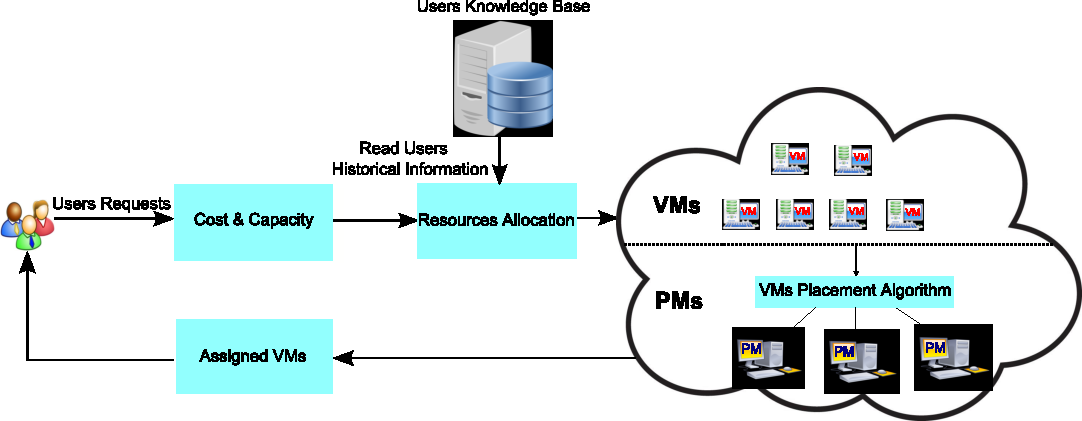
\includegraphics[width=7in]{pic/frame.pdf}
\caption{Work flow diagram showing Churn Aware Cloud Computing Framework}
\label{frame}
\end{figure*}

Our goal in this paper is to address customer churn problem in cloud computing businesses by improving the customer satisfaction while maximizing the total profit. Our problem scenario includes customers with certain SLAs, level of satisfaction and finding the best VMs placement strategy in cloud environment. Therefore, the related work section is subdivided into three parts, the dynamics of customer churn, retention and profitability, customer churn identification, and resource allocation and placement for profit maximization/cost minimization in cloud. 
\subsection{Customer Churn, Retention and Profitability}
%This is an example of a subsection title that needs to be changed to something we will be possibly using


A theoretical framework on customer retention and maximization of profit is presented in~\cite{lemmens2013managing}. Proposed work describes a relation between individual customer value and retention action, which is a popular and effective way to keep the customers and reduce the churn rate. Data mining models to predict customer churn in B2B along with profitability metric to maximize the profit of a retention campaign is proposed in~\cite{TamaddoniJahromi20141258}. This study concludes that model driven approach to churn management outperforms managerial heuristics. Several  important  considerations, including  the  value  of  cohorts,  types  of 
future revenue, and how to model retention and lifetime value for cloud business are explored in~\cite{cloudchurn2012}. This study shows how  churn  can  completely  undermine  a  seemingly  healthy cloud business. 


\subsection{Churn Identification}

The cloud providers need to predict and calculate the churn rate based on historical customer data. There have been several work on machine learning framework for identification and prediction of churners in a business. The framework in ~\cite{fasanghari2011customer} relies on a local linear model tree to identify and predict future churners in an iranian telecommunication companies. A neural network approach is proposed in~\cite{hadden2008customer}. In \cite{buckinx2007predicting}, a multiple linear regression model is developed to predict a customer’s behavioral loyalty by using the transactional database. 
Another machine learning framework to address churn problem in telecommunication is proposed in~\cite{obiedat2013customer}       .  The technique proposed in this work uses a hybrid genetic programming method is used where first, K-means  clustering  is used  to  filter outliers and non  representative  customer  behaviors  from training data, then Genetic  Programming  is  applied  to 
build classification trees to distinguish churners from  non  churners. It is to be noted that our work uses a Bayesian classifier approach which is computationally efficient.
 
\subsection{Economics in Resource Allocation and Placement}
This subsection describes some notable work on economics in resource allocation and placement. Cloud computing related work on improvement in customer satisfaction is presented in~\cite{chen2011tradeoffs} where customers’ satisfaction is abstracted and quantified in an auction framework.  Workload model and the failure correlations to redirect requests to appropriate cloud providers is considered in~\cite{javadi2012hybrid}, furthermore, evaluation of performance and monetary cost of the proposed policies is performed. Resource allocation strategy in cloud computing clusters and physical machines is proposed to maximize the overall profit in~\cite{goudarzi2011maximizing}. A combinatorial auction-based resource allocation protocol is proposed in~\cite{das2005combinatorial} and its economic efficiency and its effect on the system performance is computed. Deadline aware workflow scheduling algorithim is proposed in~\cite{abrishami2013deadline}. Algorithms to optimize work-flow scheduling and to reduce total resource provisioning cost are proposed in~\cite{chaisiri2010robust}. The extension of the work that includes various computation resources is found in~\cite{chaisiri2012optimization}. Research on billing strategies that involve various cloud computing resources ins presented in~\cite{li2012research}.

Our resource allocation and placement strategy includes both, interference and operation overhead~\cite{lin2012interference, li2013performance} of virtual machines. Interference and operation overheads affect practical VM placement on physical machines, therefore, it affects the cost.
%In the paper \cite{lin2012interference}, they looked into IAVMP problem and offer a heuristic algorithm to solve it. Li et al. \cite{li2013energy} focused on online VMs placement to minimize the total consumption and to decrease the number of fragments. Finally, when we considered response time, a paper \cite{li2014task} mentioned an algorithm of scheduling, and researchers divided the task into several parts and allocate them.





\section{Big Data Attacks and Detection Mechanisms}
\label{attacks}

\subsection{Simulation set-up}
In our experiment, the value of coefficients $b$ and $c$ in overhead functions (equation ~\ref{operationover} and ~\ref{intereferenceover}) are 0.05 and 1.5 respectively. The value of coefficient $\varphi$  in retention function (equation~\ref{eq:retention}) is 1. And the value of coefficients $\alpha$ and $\beta$ in utility function (equation~\ref{eq:reveneue})   are 100 and 60 respectively.
To demonstrate our proposal, the number of customers (i.e. number of VMs) ranges from 500 to 3000. 

We consider two types of datasets as described below:

\textit{Real Data Set:} Large dataset of a telephone company available at the Teradata Center at duke university\footnote{http://www.fuqua.duke.edu/} is used to compute real life churn rate (It is labeled as Telecom in our results). The dataset contains the information of more than 100000 customers. See Table~\ref{table1} for some sample features. We assume that data set for cloud service customers would be similar. 
 
\textit{Synthetic data:} Datasets representing various churn rates are generated by using Gaussian distribution function. We believe synthetic data represents variation of resource requests from users as observed in cloud computing industry.  


%\begin{table}[!h]
%\caption{Possible Cloud Customer Data (inspired by Telecom user dataset)}
%\label{table1}
%\centering
%\begin{tabular}{|p{2.4cm}|p{1.1cm}|p{2cm}|p{1.5cm}|}
%\hline
%\hline
%Features&Data type&Descrition&Example\\
%\hline
%\hline
%sbscrp\_id&number&customer ID&0019164958, 0019164958...\\
%\hline
%BIRTH\_DT&date&Date of birth&19610425, 19440112...\\
%\hline
%zip\_code&number&zip code&08648, 20774...\\
%\hline
%bill\_month&int&bills of customers&15219, 15249...\\
%\hline
%plan\_chosen&int&telephone plan&1, 2, 3, 4\\
%\hline
%total\_minute\_qty\_sum&int&total call minutes&57, 21...\\
%\hline
%churn&int&churner or non-churner&0, 1\\
%\hline
%\end{tabular}
%\end{table}

\begin{figure}[!h]
\centering
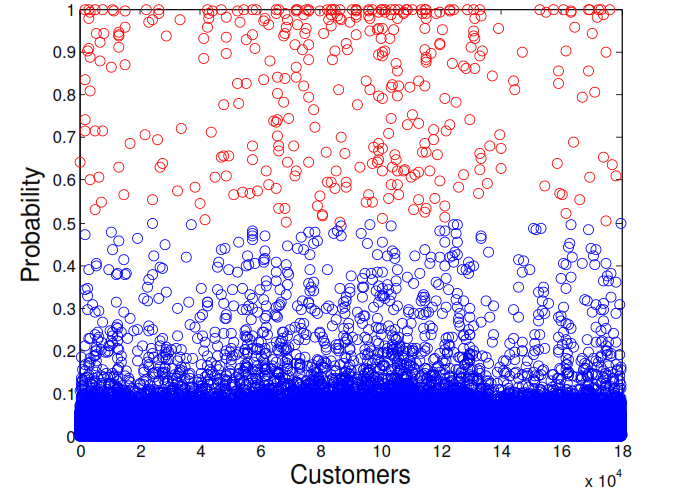
\includegraphics[scale = 0.52]{pic/churn.png}
\caption{ Churner (red bubbles) and non-churner (blue bubbles) identification in Telecom Data using naive bayesian method, churn rate = 3\%}
\label{Churnerclassification}
\end{figure}

\subsection{Results}

\subsubsection{Churner Classification} Naive Bayesian classifier is applied on Telecom dataset and result is shown in Figure~\ref{Churnerclassification}. Classifier is trained by using labeled data which is 10\% of the overall data set. We found Naive Bayesian classifier to be highly accurate. Moreover, using the classifier, churn rate in Telecom data is found to be 3\%. We believe cloud computing data would be similar to telecom customer data therefore, to demostrate our proposal on real data, we chose to  include results using Telecom data where different sample sizes are achieved by performing uniform sampling on the overall data. 

\subsubsection{Homogeneous VMs, Homogeneous PM}
In this scenario, all the requested VMs are same capacity of 0.2GHz. All PMs are of same capacity (= 3GHz, dual core) and they all costs the same (= 16).  Based on different churner rate, we use more PMs to give retention to large number of churners. Figure \ref{result1}(a) shows the number of PM used under various sizes of VMs (customers) for different churn rates. We observe a linear increase in number of PM used as number of VM increases. Small churn rates such as 0.03/0.05 can be handled by little to no increase in turned on PMs. However, for large churn rates more PMs need to be turned on. Figure \ref{result1}(b) shows the corresponding results on profit. Profit follows the similar trend where cloud service provide  
rs will have to sacrifice more revenue to tackle high churn rate.
\begin{figure*} [!htp]
  \centering
  \subfigure[Number of Physical Machines]{\label{outcastdroptail}
   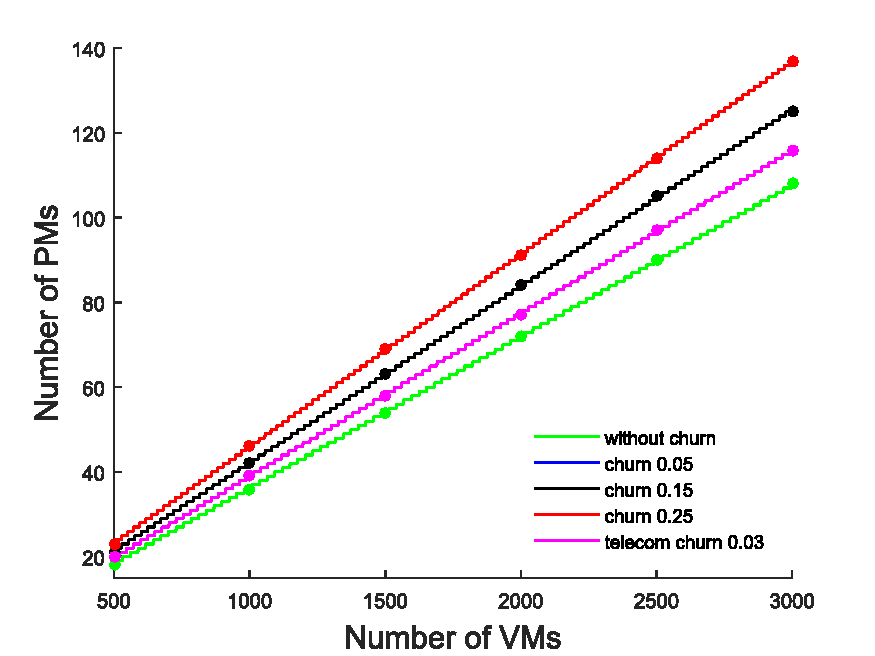
\includegraphics[width=0.4\textwidth]{pic/result1.pdf}} \quad
  \subfigure[Profit]{\label{outcastred}
   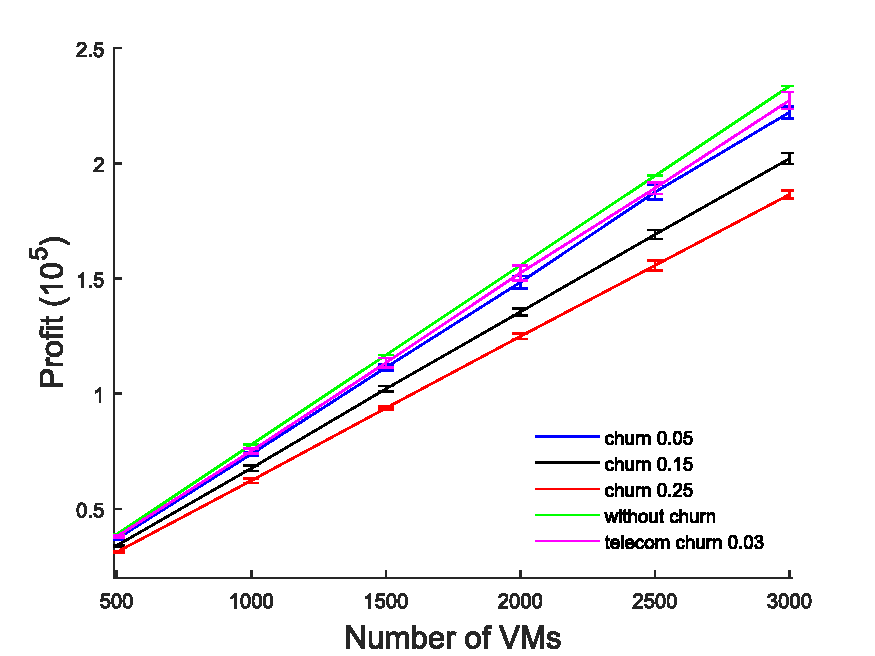
\includegraphics[width=0.4\textwidth]
{pic/profit1.pdf}} 
  \caption{Number of physical machines used and cloud service provider profit for homogeneous VMs (0.2GHz) and homogeneous PM (3GHz, dual core)  }
  \label{result1}
\end{figure*}


\subsubsection{Heterogeneous VMs, Homogeneous PMs}
In this scenario, all the requested VMs are of different capacities following a Gaussian distribution in capacity range from 0.25GHz to 1.5GHz whereas PMs are still the same as in the previous case. The trend in Figure~\ref{result2}(a) and Figure~\ref{result2}(b) is same as shown in previous section. However, because VMs request sizes have large variations, we observe profit has dropped significantly which is also evident by higher number of physical machine used as compared to previous case. Interestingly, we do not see an exact linear increase in either profit or number of PMs used as number of VM increases. The trend suggests that in the case of high number of customers, a little increase in customers with the same churn rate can be handled with little to no cost to the company. Results for churn and without churn show that such adaptation of the system is rooted in the integration of churn aware allocation and linear programming framework of VM placement. 

\begin{figure*} [!htp]
  \centering
  \subfigure[Number of Physical Machines]{\label{outcastdroptail}
   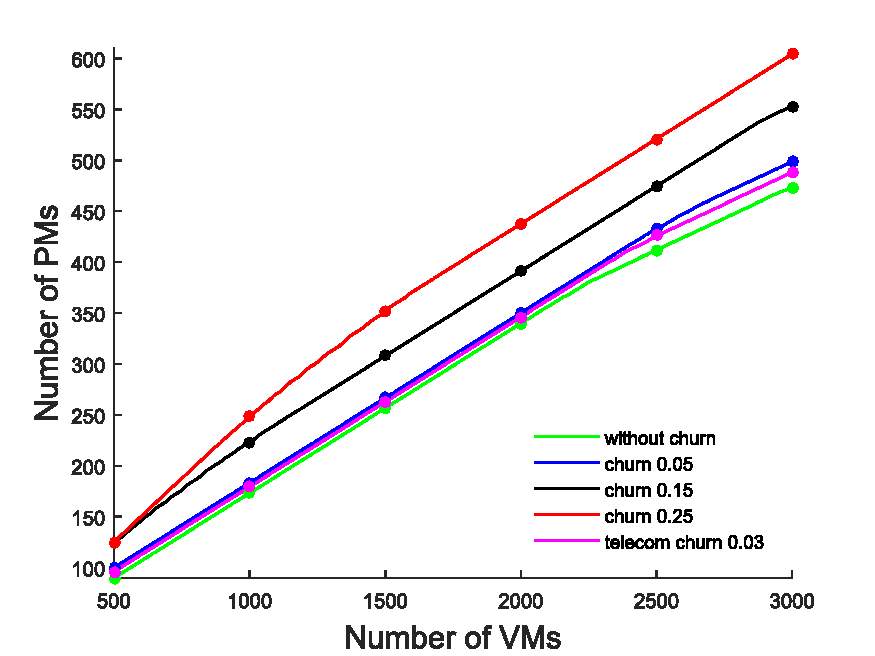
\includegraphics[width=0.4\textwidth]{pic/result2.pdf}} \quad
  \subfigure[Profit]{\label{outcastred}
   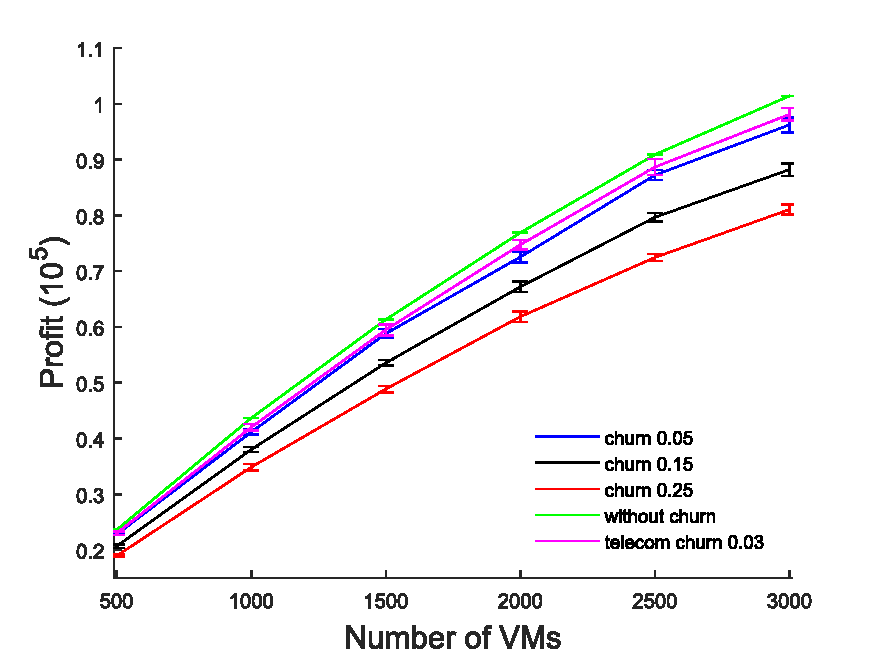
\includegraphics[width=0.4\textwidth]
{pic/profit2.pdf}} 
  \caption{ Number of physical machines used and cloud service provider profit for heterogeneous VMs and homogeneous PM (3GHz, dual core)  }
  \label{result2}
\end{figure*}


\begin{figure*} [!htp]
  \centering
  \subfigure[Number of Physical Machines]{\label{outcastdroptail}
   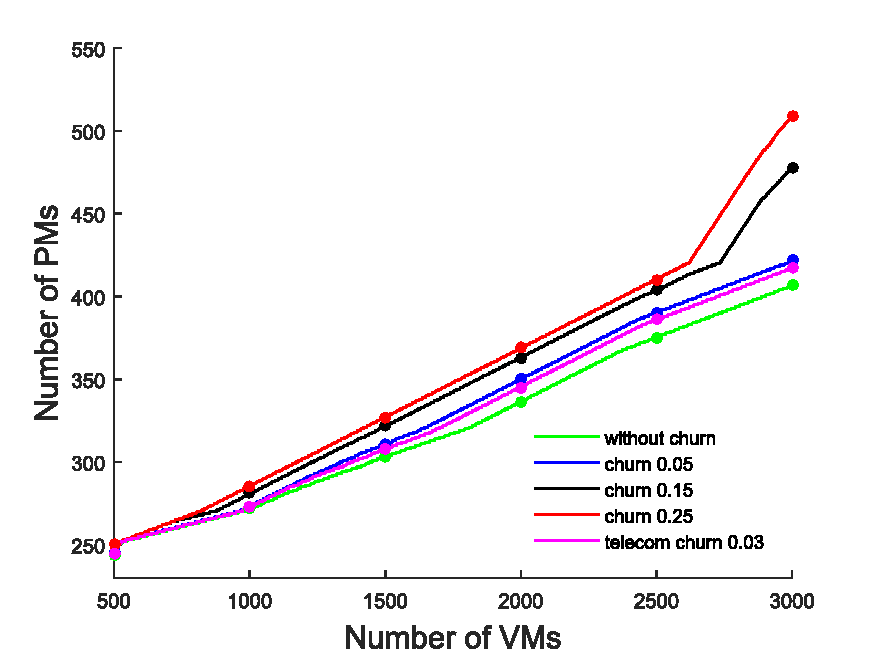
\includegraphics[width=0.4\textwidth]{pic/result3.pdf}} \quad
  \subfigure[Profit]{\label{outcastred}
   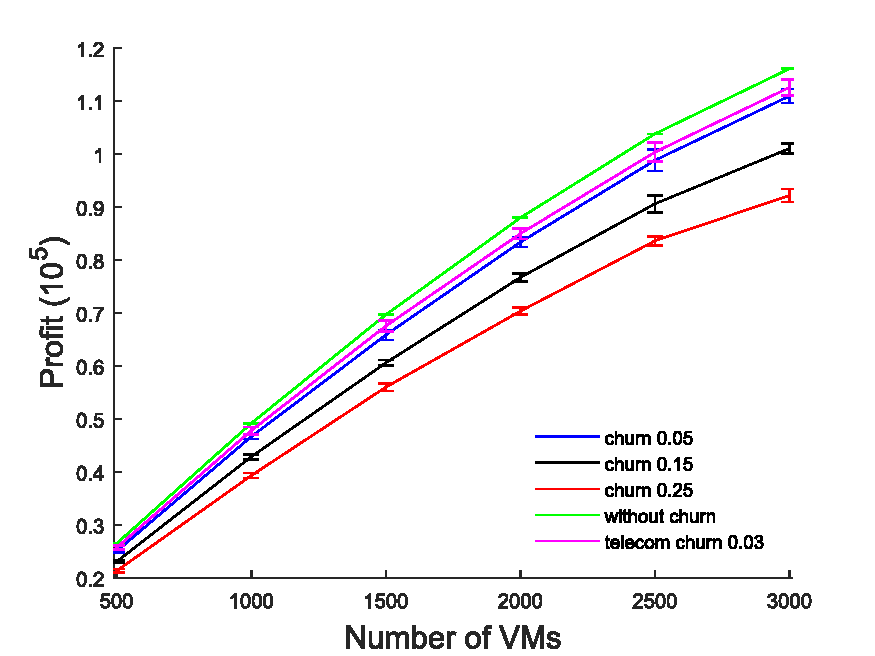
\includegraphics[width=0.4\textwidth]
{pic/profit3.pdf}} 
  \caption{ Number of physical machines used and cloud service provider profit for heterogeneous VMs and heterogeneous PMs  }
  \label{result3}
\end{figure*}

\subsubsection{Heterogeneous VMs, Heterogeneous PMs}
%Next case we considered the method to assign VMs into appropriate physical machines.The companies and service providers could have enough PMs for cloud computing, those PMs could be multifarious. For example, Amazon EC2 has many series physical infrastructures for cloud service, users can based their requirements to match and apply different VMs, some of them have strong CPU capacity for computing while some VMs are created with a low CPU capacity but a large hard disk space in order to store big data. Some service provider could have all same PMs and the VMs are also fixed. Based on section III, V and VI, we assume we have these PMs, and parameters in the below table \ref{table}. 

\begin{table}[!htp]
\caption{different Classes of Physical Machines used in the case of Heteregenous PMs}
\label{table}
\centering
\begin{tabular}{c|c|c|c|c}
\hline
\hline
Class&Capacity(GHz)& \# of Core &Cost& Machine count\\
\hline
\hline
A&3.0&8&100&20\\
\hline
B&2.7&6&85&30\\
\hline
C&2.5&6&70&50\\
\hline
D&3.0&4&60&100\\
\hline
E&2.5&4&55&150\\
\hline
F&2.5&2&40&200\\
\hline
G&2.0&2&20&200\\
\hline
H&1.5&2&10&250\\
\hline
\end{tabular}
\end{table}
The companies and service providers have PMs that are multifarious in nature to meet the diverse cloud customers. To simulate this scenario,  we use 8 classes of PMs and a total of 1000 PMs as shown in Table~\ref{table}. These PMs represent diverse capacity and costs found in a typical data centers (for example, Amazon EC2 has physical machines with diverse capacity and costs). The result for scenario is presented in Figure~\ref{result3}. The trend is similar as that of (Heterogeneous VMs, Heterogeneous PMs) case. However, we do observe a steep rise in number of PMs with the increase in VMs for higher churn rate, 0.15 and 0.25. The reason for this offshoot is with higher churn rate comes the more budget for retention action, therefore, higher added capacities for churners. Moreover, under this scheme, since machines with higher performance/cost runs out first the leftover machines being smaller in size putting a cap on number of VMs it can accommodate, therefore, we see a rise in number of machines used. However, profit trend is unaffected by it that reflects a good performance/cost ratio of machines in cloud datacenter. 

   

% An example of a floating table. Note that, for IEEE style tables, the 
% \caption command should come BEFORE the table. Table text will default to
% \footnotesize as IEEE normally uses this smaller font for tables.s
% The \label must come after \caption as always.
%


%Obviously, after the rank H has the highest Cost performance so we plan to use H fist, if Hs are not enough, then As come second, so on and so force until all VMs are placed on.
 %In our experiment,  Then, we use two algorithms for these 3000 VMs to place on 1000 PMs, the result is shown in figure x.
 







\section{Standard Prevention Mechanisms}
\label{prevention}
\subsection{Churn Aware Resource Allocation}

\subsubsection{Churner Classification}
Naive Bayesian Classifier is chosen because it is computationally efficient and degree of churn is equal to the posterior probability, however, other approaches, such as regression, decision trees, neural networks etc. can also be used. Machine learning framework using Naive Bayesian classifier is shown in Figure~\ref{classification}.
\begin{figure}[!h]
\centering
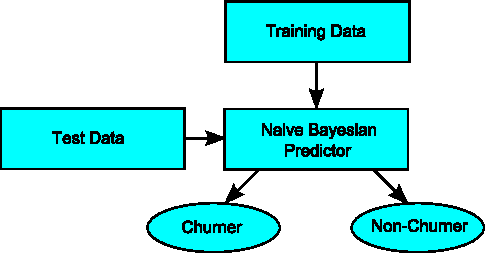
\includegraphics[width=3.5in]{pic/classification.pdf}
\caption{Machine learning framework for churner classification using Naive Bayes classifier}
\label{classification}
\end{figure}

\begin{table}[!h]
\caption{Cloud Customer Data (inspired by Telecom user dataset)}
\label{table1}
\centering
\begin{tabular}{|p{1.1cm}|p{3cm}|p{3cm}|}
\hline
\hline
Data type&Description&Example\\
\hline
\hline
number&customer ID&019164958, 019164958..\\
\hline
date&Date of birth&19610425, 19440112...\\
\hline
number&zip code&08648, 20774...\\
\hline
int&bills of customers&15219, 15249...\\
\hline
int&service plan&1, 2, 3, 4\\
\hline
int&total duration of service&57, 21...\\
\hline
int&churner or non-churner&0, 1\\
\hline
\end{tabular}
\end{table}
Attributes associated with customers of cloud service providers may look like as shown in Table~\ref{table1}. Customer data is treated as vectors denoted as $X=\{x_1,x_2,...,x_n\}$  with $n$ attributes. Naive Bayesian Predictor is trained by feeding the vectors X and labels. The trained predictor maps vectors $X_i$ to label $Y_j$ for every $i^{th}$ feature in customer data and for every class $j$. And then we compute probability $P(X_i,i\in n|Y_j, j\in m)$, which contain n features and m classes, in this case m has two values that are 1 and 0 representing classes $churn$ and $non-churn$ respectively. According to Bayes' theorem:
\begin{equation*}
P(Y)P(X|Y)=P(X)P(Y|X)
\end{equation*}
$P(X|Y)$ donate to probability of each feature given class $Y$,and $P(Y|X)$ is the probability of each class given feature $X$. The class for which we get maximum value $\sum_{i=1}^n P(Y_j|X_i)$ the customer belongs to that class. In the case of two classes, $churn$ and $non-churn$,  if the probability of $churn$ is higher than probability of $nonchurn$, then the customer belongs to the class $churn$. Furthermore, if a customer belongs to class $churn$ then the degree of churn is computed as below,
\begin{equation}
D_i=\sum_{i=1}^n P(Class=churn|X_i) 
\label{eq:degchurn}
\end{equation}

\subsubsection{Resources Allocation}
Cloud users pay for cloud resources according to equation~\ref{eq:reveneue}. If a user is identified as churner, retention action according to equation~\ref{fixed} is computed. Moreover, to improve churner satisfaction level, additional resources is given according to retention strategy as described in last section. The churner will get an added capacity, therefore, final capacity for some churner $i$ is computed as below:
\begin{equation*}
O_{i}=\dfrac{p_{i}+RC_{i}-\beta}{\alpha}
\end{equation*}

\subsection{Virtual Machine Placement}
 Virtual machines characterized by allocated resources are placed on physical machines. In our work, we assume that one PM can host multiple VMs. For demonstration purposes, we assume a single VM represents a single user. It is to be noted that our work can be easily expanded to multiple VM request per user.
\subsubsection{Linear Programming Formulation}
Every physical machine $j$ is characterized by 2-tuple, $\{Q_j,C_j\}$ where $Q_j$ and $C_j$ are capacity and costs associated with a physical machine respectively. Virtual machine placement problem is formulated as linear programming problem for profit maximization as below: \\


$Maximize:$
\begin{equation}
\label{Pro}{(\sum_{i=1}^n (\alpha O_i+\beta))-\sum_{j\in TO} C_j }
\end{equation}

$Constraints:$
\begin{equation}
\label{Con1}
\sum_{i=1}^n\theta_{ij}=1 \forall j
\end{equation}

\begin{equation}
\label{Con2}
Q_j\geqslant \sum_{i=1}^n\theta_{ij} O_i+H_j
\end{equation}

The first part in equation~\ref{Pro} is revenue and the second part is cost of runningm physical machine. Since there is flat cost associated with each physical machines, our profit maximization problem becomes cost minimization problem. 
The first constraint states that one VM is allocated to one PM (equation~\ref{Con1}). Second constraint (equation \ref{Con2}) states that capacity of VMs and overhead should not exceed the total capacity of a PM (refer equation~\ref{totaloverhead} for $H_j$). 


%In this bar chart, the PPR decreases from left to right. So that mean the more PMs close to left turns on the less money will be cost. For determining which PMs need to be turned on, there are two algorithms which are First-Fit and Best-Fit.

%\subsection{Placement Algorithm 1}
%Since cloud provider got the capacity of each VM, and capacity of PMs are also known, so it just puts VMs into these PMs based on the rank. In this case, the PM10 (35GHz, 20\$) will be used first. From left to right, so the next is PM8, then PM9, so on and so force. Till all VMs are placed on PMs, then cloud provider will know which PMs need to be turned on.
%\begin{algorithm}
 %\caption{Placement Algorithm 1}
 %\begin{algorithmic}[1]
 %\renewcommand{\algorithmicrequire}{\textbf{Input:}}
 %\renewcommand{\algorithmicensure}{\textbf{Output:}}
 %\REQUIRE Physical machines(PM) with {cost of running each PM, number of cores, and core frequency(GHz)}, virtual machines(VM)
 %\ENSURE  running Physical machines, and total cost of running Physical machines
 %\STATE calculate the cost performance of PMs
 %\STATE rank PMs according to cost performance
 %\\ \textit{LOOP Process}
  %\FOR {each VM i}
  %\FOR {each PM j}
  %\STATE check if there is a core in the CPU can process the VM
  %\STATE occupy = Occupied\_PM(j)+VM(i)+overhead
  %\IF {occupy<PM(i)}
  %\STATE assign the VMi to the PMj
  %\ENDIF
  %\ENDFOR
  %\ENDFOR
  %\STATE compute the cost of running physical machine
 %\end{algorithmic} 
 %\end{algorithm}
 
\subsubsection{Best Fit Heuristics}

  \begin{algorithm}
 \caption{VM Placement Algorithm}
 \begin{algorithmic}[1]
 \renewcommand{\algorithmicrequire}{\textbf{Input:}}
 \renewcommand{\algorithmicensure}{\textbf{Output:}}
 \REQUIRE Physical Machines (PMs) with {cost of PMs, number of cores, and core frequency (GHz)}, Virtual Machines (VMs)
 \ENSURE  Virtual Machines assignment to Physical machines, and profit
 \STATE calculate the cost - performance ratio of PMs
 \STATE rank PMs according to cost - performance ratio
 \\ \textit{LOOP Process}
  \FOR {each $PM_j$}
  \STATE check if there is a core that can process VMs
  \STATE check occupied size of $PM_j$
  \FOR{each $VM_i$}
  \STATE find the maximal $VM_i$ that can be assigned to $PM_j$
  \STATE occupy = Occupied\_$PM_j$+$VM_i$+overhead
  \IF {occupy$< PM_j$}
  \STATE assign the $VM_i$ to the $PM_j$
  \ENDIF
  \ENDFOR
  \ENDFOR
  \STATE compute the Profit 
  \STATE return profit, run PMs
 \end{algorithmic} 
 \end{algorithm}
%For a single PM, it can be used for multiple VMs. Actually we are going to divide a PM into many VMs, the physical resources support multiple VMs. However, we can abstract this problem to a Bin Packing algorithm by an opposite strategy. Totally, a PM has certain physical resources which VMs are not. VM resources are various due to the different requirements from customers, and VMs use the certain physical resources form PMs. Based on these theories, we assume PMs are bags, and VMs are the things need to be putted into these bags. Obviously, each VM has different capacity that meaning they have diverse weights. Meanwhile, PMs also have different capacities and costs. We have mentioned above, to minimize summarized cost is equal to maximize profit because of the revenue is fixed. So to reduce the cost is to use less physical machines. But here is an issue that how do cloud provider decided to turn on which physical machines?
The optimization problem described in the last section is NP complete. In this section, we suggest a heuristics to solve this problem in linear time. Note that physical machines can be distinguished by only this 2-tuple-(${Q_j,C_j}$).  Algorithm 1 describes the solution for VM placement problem. PMs are sorted in decreasing order of performance/price ratio (PPR) given by $\frac{Q_j}{C_j}$. Then we apply best-fit heuristics to solve the linear programming problem presented in last subsection.

%Another placement strategy is called Best-Fit Algorithm, compared with First-Fit Algorithm, this one has an obvious advantage that every used core is as full as possible, system always seek the most suitable VM to place on the current core so that each core has a high-usage. If we do this way, the disadvantage point is we need to set up a monitor program to listen all current VMs and traverse all VMs to find the most suitable one, assuredly, this way may raise the manager node workload.


\section{Models}
\label{model}
\input{subtex/model}
%\subsection{Utility Function}
%\label{utility}
%\input{subtex/utility}}

\section{Conclusion}
\label{conclusion}
This paper presents a customer churn aware resource allocation and virtual machine placement framework for cloud. The proposed idea rests on a successful strategy of improving customer satisfaction levels by providing better/more services. 
The proposed framework utilizes historical customer knowledge base to identify possible churners and under a retention action policy it allocates additional resources to the dissatisfied customers. Allocated resources in the form of VM is placed on PM using a profit maximization framework. The formulated profit maximization framework uses operation as well as interference overheads. Additionally, we suggest a machine learning framework to identify churners. We show the effectiveness of our work through extensive simulation by using real life as well as synthetic data. 

This is the first work that proposes customer churn awareness in resource allocation and placement in cloud service industry. Although the processor speed is used as a capacity parameters in our work the framework is equally applicable when definition of capacity is expanded to include other resources such as storage and memory. Another limiting factor of our work is the retention action where it is not certain whether the offered retention action would be accepted by the user, therefore, our future work aims to include this consideration to offer a meaningful retention action for cloud users. Our proposed work is based on strategy that better experience/service means better satisfaction, however, estimation of improvement in satisfaction level under this strategy is better suited for cloud service providers that we leave for future . Although issue of customer churn can be addressed by considering several other vital factors in cloud computing service industry our simple proposal is an attempt to promote the research and development effort in this direction.  


%In this paper, we talk both churn rate and VMs placement, our aim to reduce the churn rate to a safe line, because high churn rate is harmful for a company or a service provider. There are many ways to reduce the churn rate, and Retention Action is a common way. From the above sections, we knew that how much Retention Action the service provider need to give to the customers under its real situation based on function $f(r_c)$. This assumed function may not accurate enough or the service provider has its own model. For this issue, we still need some more big data to test and verify it, and then we can come up with an accurate function model. Furthermore, there are two schemes we talked in section IV, but scheme 2 (Ambulatory Retention Action) is flexible, the service provider doesn’t have a budget on Retention Action, so the churn rate could be reduced more than fixed scheme, in this case, service provider can use least retention action to get a lowest churn rate and highest total profit. This paper addressed how to reduce the churn rate in cloud service, and how to place VMs for decreasing cost. Giving the retention action to customers is a good way to enhance customers’ degree of satisfaction. On the other hand, an excellent placement strategy can dramatically decrease cost of PMs, so we can get an optimal profit.






% An example of a floating figure using the graphicx package.
% Note that \label must occur AFTER (or within) \caption.
% For figures, \caption should occur after the \includegraphics.
% Note that IEEEtran v1.7 and later has special internal code that
% is designed to preserve the operation of \label within \caption
% even when the captionsoff option is in effect. However, because
% of issues like this, it may be the safest practice to put all your
% \label just after \caption rather than within \caption{}.
%
% Reminder: the "draftcls" or "draftclsnofoot", not "draft", class
% option should be used if it is desired that the figures are to be
% displayed while in draft mode.
%


% Note that IEEE typically puts floats only at the top, even when this
% results in a large percentage of a column being occupied by floats.


% An example of a double column floating figure using two subfigures.
% (The subfig.sty package must be loaded for this to work.)
% The subfigure \label commands are set within each subfloat command,
% and the \label for the overall figure must come after \caption.
% \hfil is used as a separator to get equal spacing.
% Watch out that the combined width of all the subfigures on a 
% line do not exceed the text width or a line break will occur.
%
%\begin{figure*}[!t]
%\centering
%\subfloat[Case I]{\includegraphics[width=2.5in]{box}%
%\label{fig_first_case}}
%\hfil
%\subfloat[Case II]{\includegraphics[width=2.5in]{box}%
%\label{fig_second_case}}
%\caption{Simulation results.}
%\label{fig_sim}
%\end{figure*}
%
% Note that often IEEE papers with subfigures do not employ subfigure
% captions (using the optional argument to \subfloat[]), but instead will
% reference/describe all of them (a), (b), etc., within the main caption.


% An example of a floating table. Note that, for IEEE style tables, the 
% \caption command should come BEFORE the table. Table text will default to
% \footnotesize as IEEE normally uses this smaller font for tables.
% The \label must come after \caption as always.
%
%\begin{table}[!t]
%% increase table row spacing, adjust to taste
%\renewcommand{\arraystretch}{1.3}
% if using array.sty, it might be a good idea to tweak the value of
% \extrarowheight as needed to properly center the text within the cells
%\caption{An Example of a Table}
%\label{table_example}
%\centering
%% Some packages, such as MDW tools, offer better commands for making tables
%% than the plain LaTeX2e tabular which is used here.
%\begin{tabular}{|c||c|}
%\hline
%One & Two\\
%\hline
%Three & Four\\
%\hline
%\end{tabular}
%\end{table}


% Note that IEEE does not put floats in the very first column - or typically
% anywhere on the first page for that matter. Also, in-text middle ("here")
% positioning is not used. Most IEEE journals/conferences use top floats
% exclusively. Note that, LaTeX2e, unlike IEEE journals/conferences, places
% footnotes above bottom floats. This can be corrected via the \fnbelowfloat
% command of the stfloats package.






% conference papers do not normally have an appendix

% trigger a \newpage just before the given reference
% number - used to balance the columns on the last page
% adjust value as needed - may need to be readjusted if
% the document is modified later
%\IEEEtriggeratref{8}
% The "triggered" command can be changed if desired:
%\IEEEtriggercmd{\enlargethispage{-5in}}

% REFERENCES SECTION ************************************************************************************

% can use a bibliography generated by BibTeX as a .bbl file
% BibTeX documentation can be easily obtained at:
% http://www.ctan.org/tex-archive/biblio/bibtex/contrib/doc/
% The IEEEtran BibTeX style support page is at:
% http://www.michaelshell.org/tex/ieeetran/bibtex/
\bibliographystyle{IEEEtran}
% argument is your BibTeX string definitions and bibliography database(s)
\bibliography{reference}
%
% <OR> manually copy in the resultant .bbl file
% set second argument of \begin to the number of references
% (used to reserve space for the reference number labels box)



\end{document}


